%  LaTeX support: latex@mdpi.com 
%  For support, please attach all files needed for compiling as well as the log file, and specify your operating system, LaTeX version, and LaTeX editor.

%=================================================================
\documentclass[journal,article,submit,pdftex,moreauthors]{Definitions/mdpi} 
%\documentclass[preprints,article,submit,pdftex,moreauthors]{Definitions/mdpi} 
% For posting an early version of this manuscript as a preprint, you may use "preprints" as the journal. Changing "submit" to "accept" before posting will remove line numbers.

% Below journals will use APA reference format:
% admsci, behavsci, businesses, econometrics, economies, education, ejihpe, famsci, games, humans, ijcs, ijfs, journalmedia, jrfm, languages, psycholint, publications, tourismhosp, youth

% Below journals will use Chicago reference format:
% arts, genealogy, histories, humanities, jintelligence, laws, literature, religions, risks, socsci

%--------------------
% Class Options:
%--------------------
%----------
% journal
%----------
% Choose between the following MDPI journals:
% accountaudit, acoustics, actuators, addictions, adhesives, admsci, adolescents, aerobiology, aerospace, agriculture, agriengineering, agrochemicals, agronomy, ai, air, algorithms, allergies, alloys, amh, analytica, analytics, anatomia, anesthres, animals, antibiotics, antibodies, antioxidants, applbiosci, appliedchem, appliedmath, appliedphys, applmech, applmicrobiol, applnano, applsci, aquacj, architecture, arm, arthropoda, arts, asc, asi, astronomy, atmosphere, atoms, audiolres, automation, axioms, bacteria, batteries, bdcc, behavsci, beverages, biochem, bioengineering, biologics, biology, biomass, biomechanics, biomed, biomedicines, biomedinformatics, biomimetics, biomolecules, biophysica, biosensors, biosphere, biotech, birds, blockchains, bloods, blsf, brainsci, breath, buildings, businesses, cancers, carbon, cardiogenetics, catalysts, cells, ceramics, challenges, chemengineering, chemistry, chemosensors, chemproc, children, chips, cimb, civileng, cleantechnol, climate, clinbioenerg, clinpract, clockssleep, cmd, cmtr, coasts, coatings, colloids, colorants, commodities, complications, compounds, computation, computers, condensedmatter, conservation, constrmater, cosmetics, covid, crops, cryo, cryptography, crystals, csmf, ctn, curroncol, cyber, dairy, data, ddc, dentistry, dermato, dermatopathology, designs, devices, diabetology, diagnostics, dietetics, digital, disabilities, diseases, diversity, dna, drones, dynamics, earth, ebj, ecm, ecologies, econometrics, economies, education, eesp, ejihpe, electricity, electrochem, electronicmat, electronics, encyclopedia, endocrines, energies, eng, engproc, ent, entomology, entropy, environments, epidemiologia, epigenomes, esa, est, famsci, fermentation, fibers, fintech, fire, fishes, fluids, foods, forecasting, forensicsci, forests, fossstud, foundations, fractalfract, fuels, future, futureinternet, futureparasites, futurepharmacol, futurephys, futuretransp, galaxies, games, gases, gastroent, gastrointestdisord, gastronomy, gels, genealogy, genes, geographies, geohazards, geomatics, geometry, geosciences, geotechnics, geriatrics, glacies, grasses, greenhealth, gucdd, hardware, hazardousmatters, healthcare, hearts, hemato, hematolrep, heritage, higheredu, highthroughput, histories, horticulturae, hospitals, humanities, humans, hydrobiology, hydrogen, hydrology, hygiene, idr, iic, ijerph, ijfs, ijgi, ijmd, ijms, ijns, ijpb, ijt, ijtm, ijtpp, ime, immuno, informatics, information, infrastructures, inorganics, insects, instruments, inventions, iot, j, jal, jcdd, jcm, jcp, jcs, jcto, jdad, jdb, jeta, jfb, jfmk, jimaging, jintelligence, jlpea, jmahp, jmmp, jmms, jmp, jmse, jne, jnt, jof, joitmc, joma, jop, jor, journalmedia, jox, jpbi, jpm, jrfm, jsan, jtaer, jvd, jzbg, kidney, kidneydial, kinasesphosphatases, knowledge, labmed, laboratories, land, languages, laws, life, lights, limnolrev, lipidology, liquids, literature, livers, logics, logistics, lubricants, lymphatics, machines, macromol, magnetism, magnetochemistry, make, marinedrugs, materials, materproc, mathematics, mca, measurements, medicina, medicines, medsci, membranes, merits, metabolites, metals, meteorology, methane, metrics, metrology, micro, microarrays, microbiolres, microelectronics, micromachines, microorganisms, microplastics, microwave, minerals, mining, mmphys, modelling, molbank, molecules, mps, msf, mti, multimedia, muscles, nanoenergyadv, nanomanufacturing, nanomaterials, ncrna, ndt, network, neuroglia, neurolint, neurosci, nitrogen, notspecified, nursrep, nutraceuticals, nutrients, obesities, oceans, ohbm, onco, oncopathology, optics, oral, organics, organoids, osteology, oxygen, parasites, parasitologia, particles, pathogens, pathophysiology, pediatrrep, pets, pharmaceuticals, pharmaceutics, pharmacoepidemiology, pharmacy, philosophies, photochem, photonics, phycology, physchem, physics, physiologia, plants, plasma, platforms, pollutants, polymers, polysaccharides, populations, poultry, powders, preprints, proceedings, processes, prosthesis, proteomes, psf, psych, psychiatryint, psychoactives, psycholint, publications, purification, quantumrep, quaternary, qubs, radiation, reactions, realestate, receptors, recycling, regeneration, religions, remotesensing, reports, reprodmed, resources, rheumato, risks, robotics, rsee, ruminants, safety, sci, scipharm, sclerosis, seeds, sensors, separations, sexes, signals, sinusitis, siuj, skins, smartcities, sna, societies, socsci, software, soilsystems, solar, solids, spectroscj, sports, standards, stats, std, stresses, surfaces, surgeries, suschem, sustainability, symmetry, synbio, systems, tae, targets, taxonomy, technologies, telecom, test, textiles, thalassrep, therapeutics, thermo, timespace, tomography, tourismhosp, toxics, toxins, transplantology, transportation, traumacare, traumas, tropicalmed, universe, urbansci, uro, vaccines, vehicles, venereology, vetsci, vibration, virtualworlds, viruses, vision, waste, water, wem, wevj, wild, wind, women, world, youth, zoonoticdis

%---------
% article
%---------
% The default type of manuscript is "article", but can be replaced by: 
% abstract, addendum, article, benchmark, book, bookreview, briefcommunication, briefreport, casereport, changes, clinicopathologicalchallenge, comment, commentary, communication, conceptpaper, conferenceproceedings, correction, conferencereport, creative, datadescriptor, discussion, entry, expressionofconcern, extendedabstract, editorial, essay, erratum, fieldguide, hypothesis, interestingimages, letter, meetingreport, monograph, newbookreceived, obituary, opinion, proceedingpaper, projectreport, reply, retraction, review, perspective, protocol, shortnote, studyprotocol, supfile, systematicreview, technicalnote, viewpoint, guidelines, registeredreport, tutorial,  giantsinurology, urologyaroundtheworld
% supfile = supplementary materials

%----------
% submit
%----------
% The class option "submit" will be changed to "accept" by the Editorial Office when the paper is accepted. This will only make changes to the frontpage (e.g., the logo of the journal will get visible), the headings, and the copyright information. Also, line numbering will be removed. Journal info and pagination for accepted papers will also be assigned by the Editorial Office.

%------------------
% moreauthors
%------------------
% If there is only one author the class option oneauthor should be used. Otherwise use the class option moreauthors.

%---------
% pdftex
%---------
% The option pdftex is for use with pdfLaTeX. Remove "pdftex" for (1) compiling with LaTeX & dvi2pdf (if eps figures are used) or for (2) compiling with XeLaTeX.

%=================================================================
% MDPI internal commands - do not modify
\firstpage{1} 
\makeatletter 
\setcounter{page}{\@firstpage} 
\makeatother
\pubvolume{1}
\issuenum{1}
\articlenumber{0}
\pubyear{2025}
\copyrightyear{2025}
%\externaleditor{Firstname Lastname} % More than 1 editor, please add `` and '' before the last editor name
\datereceived{ } 
\daterevised{ } % Comment out if no revised date
\dateaccepted{ } 
\datepublished{ } 
%\datecorrected{} % For corrected papers: "Corrected: XXX" date in the original paper.
%\dateretracted{} % For retracted papers: "Retracted: XXX" date in the original paper.
\hreflink{https://doi.org/} % If needed use \linebreak
%\doinum{}
%\pdfoutput=1 % Uncommented for upload to arXiv.org
%\CorrStatement{yes}  % For updates
%\longauthorlist{yes} % For many authors that exceed the left citation part

%=================================================================
% Add packages and commands here. The following packages are loaded in our class file: fontenc, inputenc, calc, indentfirst, fancyhdr, graphicx, epstopdf, lastpage, ifthen, float, amsmath, amssymb, lineno, setspace, enumitem, mathpazo, booktabs, titlesec, etoolbox, tabto, xcolor, colortbl, soul, multirow, microtype, tikz, totcount, changepage, attrib, upgreek, array, tabularx, pbox, ragged2e, tocloft, marginnote, marginfix, enotez, amsthm, natbib, hyperref, cleveref, scrextend, url, geometry, newfloat, caption, draftwatermark, seqsplit
% cleveref: load \crefname definitions after \begin{document}
\usepackage{matlab-prettifier}

%=================================================================
% Please use the following mathematics environments: Theorem, Lemma, Corollary, Proposition, Characterization, Property, Problem, Example, ExamplesandDefinitions, Hypothesis, Remark, Definition, Notation, Assumption
%% For proofs, please use the proof environment (the amsthm package is loaded by the MDPI class).

%=================================================================
% Full title of the paper (Capitalized)
\Title{A Practical Youla Gain-Tuning Framework for $H_\infty$ Controller Realization}

% MDPI internal command: Title for citation in the left column
\TitleCitation{A Practical Youla Gain-Tuning Framework for $H_\infty$ Controller Realization}

% Author Orchid ID: enter ID or remove command
\newcommand{\orcidauthorA}{0009-0009-3531-2294} % Add \orcidA{} behind the author's name
\newcommand{\orcidauthorB}{0009-0008-5166-6087} % Add \orcidB{} behind the author's name
\newcommand{\orcidauthorC}{0000-0002-7934-3457}
% Authors, for the paper (add full first names)
\Author{Ricardo Tan \orcidA{}, Siddhesh Yadav \orcidB{} and Francis Assadian *\orcidC{}}

%\longauthorlist{yes}

% MDPI internal command: Authors, for metadata in PDF
\AuthorNames{Ricardo Tan, Siddhesh Yadav and Francis Assadian}

% MDPI internal command: Authors, for citation in the left column, only choose below one of them according to the journal style
% If this is a Chicago style journal 
% (arts, genealogy, histories, humanities, jintelligence, laws, literature, religions, risks, socsci): 
% Lastname, Firstname, Firstname Lastname, and Firstname Lastname.

% If this is a APA style journal 
% (admsci, behavsci, businesses, econometrics, economies, education, ejihpe, games, humans, ijfs, journalmedia, jrfm, languages, psycholint, publications, tourismhosp, youth): 
% Lastname, F., Lastname, F., \& Lastname, F.

% If this is a ACS style journal (Except for the above Chicago and APA journals, all others are in the ACS format): 
% Lastname, F.; Lastname, F.; Lastname, F.
\isAPAStyle{%
       \AuthorCitation{Tan, R., Yadav, S., \& Assadian, F.}
         }{%
        \isChicagoStyle{%
        \AuthorCitation{Tan, Ricardo, Siddhesh Yadav, and Francis Assadian.}
        }{
        \AuthorCitation{Tan, R.; Yadav, S.; Assadian, F.}
        }
}

% Affiliations / Addresses (Add [1] after \address if there is only one affiliation.)
\address[1]{%
Department of Mechanical \& Aerospace Engineering, {University} of California, Davis, CA 95616, USA;
rstan@ucdavis.edu (R.T.); syadav@ucdavis.edu (S.Y.)}

% Contact information of the corresponding author
\corres{\hangafter=1 \hangindent=1.05em \hspace{-0.82em}Correspondence: fassadian@ucdavis.edu (F.A.)}

%\simplesumm{} % Simple summary

%\conference{} % An extended version of a conference paper

% Abstract (Do not insert blank lines, i.e. \\) 
\abstract{
Standard $H_\infty$ controller synthesis produces robust controllers with well-shaped sensitivity and complementary sensitivity transfer functions, $S$ and $T$. However, at times $H_\infty$ does not enforce strict requirements on sensitivity, in particular the desired requirement that $T$ has unity gain at DC frequency. This results in typically negligible steady-state tracking error, as the $H_\infty$ optimization produces  $T(0)\approx1$. In drive cycle applications where reference velocity profiles contain extended ramp segments, this negligible deviation is integrated over time into a growing, non-negligible bias. The conventional remedy is to augment the plant with an integrator prior to synthesis, but this increases the order of the plant model and can be inconvenient when the control designer's modeling has already been completed. This paper presents a post-synthesis gain adjustment method using Youla parameterization that corrects the DC tracking deficiency without modifying the plant or repeating $H_\infty$ synthesis. The poles and zeros corresponding to the $H_\infty$ controller’s Youla transfer function $Y$ are preserved, with a free parameter $K$ replacing the gain of $Y$. Re-calculating the controller after solving for the value of $K$ that enforces $T(0)=1$ results in a hybrid controller that retains the robustness of the original but with improved performance in ramp-input scenarios with minimal effort for the control designer. Simulation results on a vehicle speed tracking problem confirm elimination of accumulating bias while preserving robustness margins from the original $H_\infty$ design.
}

% Keywords
\keyword{$H_\infty$ control, Youla parameterization, gain tuning, control design automation} 

% The fields PACS, MSC, and JEL may be left empty or commented out if not applicable
%\PACS{J0101}
%\MSC{}
%\JEL{}

%%%%%%%%%%%%%%%%%%%%%%%%%%%%%%%%%%%%%%%%%%
% Only for the journal Diversity
%\LSID{\url{http://}}

%%%%%%%%%%%%%%%%%%%%%%%%%%%%%%%%%%%%%%%%%%
% Only for the journal Applied Sciences
%\featuredapplication{Authors are encouraged to provide a concise description of the specific application or a potential application of the work. This section is not mandatory.}
%%%%%%%%%%%%%%%%%%%%%%%%%%%%%%%%%%%%%%%%%%

%%%%%%%%%%%%%%%%%%%%%%%%%%%%%%%%%%%%%%%%%%
% Only for the journal Data
%\dataset{DOI number or link to the deposited data set if the data set is published separately. If the data set shall be published as a supplement to this paper, this field will be filled by the journal editors. In this case, please submit the data set as a supplement.}
%\datasetlicense{License under which the data set is made available (CC0, CC-BY, CC-BY-SA, CC-BY-NC, etc.)}

%%%%%%%%%%%%%%%%%%%%%%%%%%%%%%%%%%%%%%%%%%
% Only for the journal Toxins
%\keycontribution{The breakthroughs or highlights of the manuscript. Authors can write one or two sentences to describe the most important part of the paper.}

%%%%%%%%%%%%%%%%%%%%%%%%%%%%%%%%%%%%%%%%%%
% Only for the journal Encyclopedia
%\encyclopediadef{For entry manuscripts only: please provide a brief overview of the entry title instead of an abstract.}

%%%%%%%%%%%%%%%%%%%%%%%%%%%%%%%%%%%%%%%%%%
% Only for the journal Advances in Respiratory Medicine, Smart Cities and Sensors
%\addhighlights{yes}
%\renewcommand{\addhighlights}{%
%
%\noindent This is an obligatory section in “Advances in Respiratory Medicine'' and ``Smart Cities”, whose goal is to increase the discoverability and readability of the article via search engines and other scholars. Highlights should not be a copy of the abstract, but a simple text allowing the reader to quickly and simplified find out what the article is about and what can be cited from it. Each of these parts should be devoted up to 2~bullet points.\vspace{3pt}\\
%\textbf{What are the main findings?}
% \begin{itemize}[labelsep=2.5mm,topsep=-3pt]
% \item First bullet.
% \item Second bullet.
% \end{itemize}\vspace{3pt}
%\textbf{What is the implication of the main finding?}
% \begin{itemize}[labelsep=2.5mm,topsep=-3pt]
% \item First bullet.
% \item Second bullet.
% \end{itemize}
%}

%%%%%%%%%%%%%%%%%%%%%%%%%%%%%%%%%%%%%%%%%%
\begin{document}

%%%%%%%%%%%%%%%%%%%%%%%%%%%%%%%%%%%%%%%%%%
\section{Introduction}
\label{sec:introduction}
Robust control design incorporates concepts of model uncertainty, disturbances, and unmodeled dynamics in order to design controllers that ensure stability and performance despite uncertainty. Each source of potential degradation of control can be mitigated via loop-shaping, where the controller is designed to ensure that the model's closed-loop sensitivity, complementary sensitivity, and Youla transfer functions ($S$, $T$, $Y$ respectively) have characteristics that ensure both robustness and performance, which are the following \citep{assadian2022robust}:
\begin{itemize}
\item $T$ is exactly 0 dB in low frequencies to track reference signals and low in high frequencies to attenuate high frequency unmodeled dynamics and sensor noise.
\item $S$ is low in low frequencies to attenuate disturbance and parameter variation effects.
\item $Y$ is low in high frequencies to limit actuator jitter resulting from sensor noise.
\item The maximum magnitude of $S$ is as close to 0 dB as possible, as this relates to system robustness.
\item The maximum magnitude of $Y$ is as low as feasible, as this determines the required actuator effort.
\end{itemize}

In $H_\infty$ synthesis, the above characteristics are achieved by finding the controller that minimizes the maximum magnitude of any entry in the vector \([W_pS, W_dT, W_uY]^T\) across all frequencies. The $W_p, W_d,$ and $W_u$ weighting transfer functions are approximately the inverse of the desired shapes for $S$, $T$, and $Y$ respectively with regards to the goals of loop-shaping, thereby giving the $H_\infty$ synthesis algorithm a cost function that naturally targets the desired loop shapes.

This makes the technique of $H_\infty$ synthesis a powerful framework for constructing controllers that minimize worst-case gain from disturbances to regulated outputs \citep{zhou1996robust, skogestad2005multivariable}. For the control designer, $H_\infty$ synthesis is a convenient method of indirectly designing robust controllers. Once a plant model $G_P$ has been determined, the control designer tunes the controller by adjusting the cost weighting functions $W_p$, $W_d$, and $W_u$, representing the designer's goals for the closed-loop performance, both in achieving the desired overall loop shapes for robustness and performance as well as the specific crossover frequency, transfer function slopes, and magnitudes at specific frequency ranges.

While it can be convenient to adjust weights rather than the controller directly, the output of $H_\infty$ synthesis does not strictly enforce loop-shaping goals since it only is aware of its cost function. The goal under current consideration is that the complementary sensitivity function, which, among other metrics, describes the ratio of the regulated output to the input reference signal, has unity gain at zero frequency (DC gain), or $T(0) = 1$ \citep{assadian2022robust}. For many cases, the output of $H_\infty$ synthesis results in $T(0) \approx 1$, for example $T(0)=0.99985$ as observed for the system in \citep{tan2025scaling}. Depending on the scenario, $T(0)$ can be either slightly below $1.0$, resulting in undershoot, or slightly above $1.0$, resulting in overshoot. Using the example of $T(0)=0.99985$, this results in a steady-state error of only $0.015\%$ for a step input which is often more than acceptable. However, in cases such as the drive cycle input used in \citep{tan2025scaling}, a reference signal that includes prolonged periods of ramping input results in the $0.015\%$ undershoot being integrated and resulting in the regulated output drifting over time.

Fine-tuning the $H_\infty$ output can be inconvenient, requiring an iterative process to tweak the input weights or requiring modifications to the plant model. The typical method used to enforce $T(0)=1$ would be to augment the plant model with an integrator \citep{seatzu2008Hinfint}, naturally enforcing $T(0)=1$. However, the selection of weighting functions for the $H_\infty$ solver must be non-trivially adjusted to account for the effect of the integrator on the plant model, where the compensation on the weighting functions changes depending on the dynamics of the original plant. This introduces a second layer of iteration if the augmentation is performed later in the controller design workflow. In addition, augmentation increases the order of the plant which will typically increase the order of the resulting controller as well, if the order of weighting functions is held constant.

A relevant iterative Youla parameterization design method was implemented in \citep{hu2025YK}, where the flexibility of Youla parameterization is utilized in order to perform loop-shaping at specific frequencies of the system. The iterative method is used in order to tune high-order controllers by modifying the existing, or previous-iteration, controller in a manner that maintains stability and achieves the desired closed loop transfer function characteristics.

The method described in this paper is a post-synthesis adjustment to the $H_\infty$ output using Youla parameterization techniques that allows for strict enforcement of $T(0)=1$ in an intuitive, easy to implement manner that is well-adapted to implementation in programming languages. Part of the benefit of our method is that the post-synthesis adjustment only requires a single scalar Youla shaping parameter and can be performed in a single step, compared to the iterative process of \citep{hu2025YK}, making the adjustment of $H_\infty$ controllers simple to implement. The hybrid method is referred to here as \textbf{Youla-H synthesis}.

When viewed from the perspective of controller design with Youla parameterization from scratch, it is much easier with Youla-H to achieve a robust controller when starting with the output of $H_\infty$ rather than attempting to select a pole/zero structure with no prior information.

%%%%%%%%%%%%%%%%%%%%%%%%%%%%%%%%%%%%%%%%%%
\section{Methods}
\label{sec:methods}
\subsection{Notation}
The standard transfer functions \citep{assadian2022robust} used throughout are defined below.

\begin{itemize}
\item \(G_P\)---plant transfer function.
\item \(G_C\)---controller transfer function.
\item \(L=G_CG_P\)---open-loop transfer function/return ratio, represents open-loop system response to reference input.
\item \(T=L/(1+L)\)---complementary sensitivity transfer function, relates to closed-loop reference tracking relative to reference input.
\item \(S=1/(1+L)\)---sensitivity transfer function, relates to closed-loop disturbance and plant parameter variation sensitivity.
\item \(Y=G_C/(1+L)\)---Youla transfer function, relates to closed-loop actuator effort relative to reference input.
\item $W_p$---cost weight transfer function on $S$ for $H_\infty$.
\item $W_d$---cost weight transfer function on $T$ for $H_\infty$.
\item $W_u$---cost weight transfer function on $Y$ for $H_\infty$.
\end{itemize}

The subscripts used throughout are:
\begin{itemize}
\item H---corresponds to $H_\infty$ transfer functions.
\item YH---corresponds to hybrid Youla-H transfer functions.
\end{itemize}

\subsection{Gain Tuning}
Equation \ref{eq:YH} describes the generalized $Y$ transfer function that would be output by the initial $H_\infty$ synthesis in zero-pole-gain (ZPK) form.
\begin{equation} \label{eq:YH}
Y_H(s) = K_H \frac{\prod_{i=1}^{n} (s + z_i)}{\prod_{j=1}^{m} (s + p_j)}
\end{equation}

The hybrid Youla-H $Y$ transfer function is given in Equation \ref{eq:YYH1}, where $K_{YH}$ is a free scalar parameter that has not yet been determined, but the values of $z_i$ and $p_i$ are the same as in the $H_\infty$ case.

\begin{equation} \label{eq:YYH1}
Y_{YH}(s) = K_{YH} \frac{\prod_{i=1}^{n} (s + z_i)}{\prod_{j=1}^{m} (s + p_j)}
\end{equation}

Alternatively, $Y_{YH}$ can be described in terms of $Y_H$, $K_H$, and $K_{YH}$.

\begin{equation} \label{eq:YYH2}
Y_{YH}(s) = \frac{K_{YH} }{K_{H}}Y_H(s)
\end{equation}

Note that since $T=L/(1+L)$ and $Y=G_C/(1+L)$, $T=G_PY$. Equation \ref{eq:T0} shows the enforcement of strict tracking performance.
\begin{equation} \label{eq:T0}
T_{YH}(0) = 1 = G_P(0)Y_{YH}(0) = \frac{K_{YH}}{K_{H}}Y_H(0)G_P(0) = K_{YH}G_P(0)\frac{\prod_{i=1}^{n} z_i}{\prod_{j=1}^{m} p_j}
\end{equation}

This resolves into equation \ref{eq:KYH}, setting the exact numeric value for $K_{YH}$.
\begin{equation} \label{eq:KYH}
K_{YH} = \frac{K_H}{Y_H(0)G_P(0)}= \frac{1}{G_P(0)}\frac{\prod_{j=1}^{m} p_j}{\prod_{i=1}^{n} z_i} 
\end{equation}

Setting $K_{YH}$ in this manner algebraically enforces $T(0)=1$ and, by extension, $S(0)=0$. Since $G_C=Y/S$, this indicates that $G_C(0)\rightarrow\infty$ which corresponds to at least one pure integrator in the final controller.

This method assumes $G_P(0) \neq 0$ and $Y(0) \neq 0$. If $G_P(0) = 0$, the plant has zero DC gain, making $T(0) = G_P(0)Y(0) = 0$ for any finite $K_{YH}$. Strict DC tracking is then unachievable through gain adjustment alone, and the Youla-H method does not apply. If $Y(0) = 0$, the $H_\infty$-synthesized Youla transfer function contains a pure differentiator, which again causes $T(0) = G_P(0)Y(0) = 0$ for any finite $K_{YH}$. In either case, the designer must revisit the plant model, weighting function selection, or the entire control methodology before potentially applying the Youla-H method.

\section{Plant Models}
The first-order plant shown in Figure \ref{fig:Youla_plant} and Equation \ref{eq:Gp} is that used in \citep{tan2025scaling}, which was used to design drive controllers for a non-linear vehicle drivetrain model. 

\begin{figure}[H]
%    \centering
    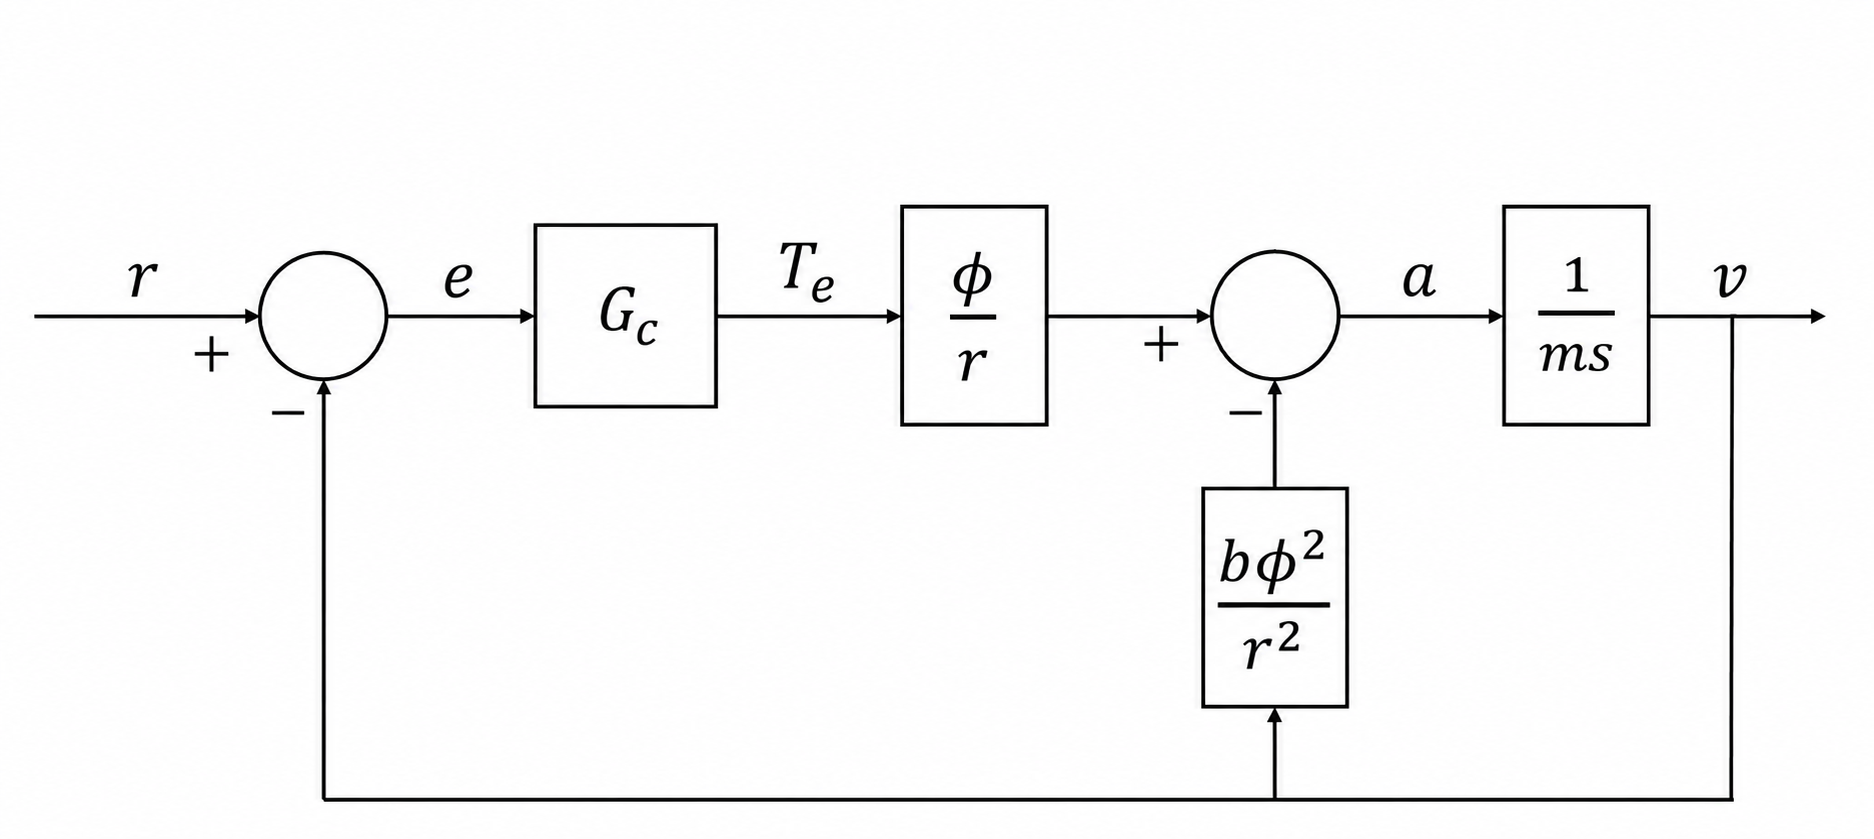
\includegraphics[width=1\linewidth]{Figures/YoulaPlant.png}
    \caption{First-order linear plant model, controller, and feedback loop.}
    \label{fig:Youla_plant}
\end{figure}

Figure \ref{fig:Youla_plant} shows the controller $G_C$, which is not part of the plant but that outputs the engine torque $T_e$, being transformed through the gear ratio, $\phi$, and the tire radius, $r$, into the driving acceleration on the vehicle. This acceleration is dampened by the $b\phi^2/r^2$ term, which represents the effect of motor friction transformed through the drivetrain. Finally, the net acceleration, $a$, is divided by the effective vehicle mass, $m$, and integrated in order to output the vehicle velocity, $v$, which is the tracked signal in the system. This linear plant model is a simplified subset of the dynamics that are modeled in the full non-linear simulation. This simplified model is used only to design controllers which, due to the robust nature of loop-shaping methods, still produces effective controllers for the nonlinear simulation used in \citep{tan2025scaling}. The torque conversion, motor friction conversion, and mass / integration blocks of Figure \ref{fig:Youla_plant} comprise the plant, $G_P$, shown in Equation \ref{eq:Gp}.

\begin{equation} \label{eq:Gp}
G_{P} = \frac{v}{T_e} = \frac{\frac{\phi}{mr}}{s+\frac{b\,\phi^2 }{m\,r^2}}
\end{equation}

For the purposes of this paper, the vehicle parameters chosen are the scaled-down parameters for the test model built in \citep{tan2025scaling}. The plant numerically reduces down to Equation \ref{eq:Gp_numerical}.

\begin{equation} \label{eq:Gp_numerical}
G_{P} = \frac{22.624}{s+0.0000432}
\end{equation}

Note that this is an exceedingly simple plant model. Despite this, the $H_{\infty}$ synthesis was not observed to produce exactly  $T(0)=1$ for any of the combinations of weighting functions that were tested, though it was not a rigorous search. As mentioned in the Introduction, a common method of compensating for the error in reference tracking is to augment the plant state space such that a pure integrator is produced by the controller. Instead, the hybrid Youla-H method is used in this paper in order to enforce strict tracking as a simple-to-implement alternative. If the Youla-H method had been utilized at the beginning of controller design, the weight selection process would have been much faster since exploration to find a controller with a better $T(0)$ value would not have been necessary. Further, work considering augmenting the plant with an integrator would not be necessary either.

At the end of the Results section, a second plant will be used to demonstrate a scenario where the Youla-H method applies even with an easier $H_\infty$ optimization. See Section \ref{sec:Alternate} for details.

%%%%%%%%%%%%%%%%%%%%%%%%%%%%%%%%%%%%%%%%%
\section{Results}
Bode plots are used to inspect the closed-loop transfer functions of the original $H_{\infty}$-produced controller and the hybrid Youla-H controller, using the linear plant transfer function. Afterwards, tracking error results are shown produced from the same nonlinear drivetrain model used in \citep{tan2025scaling}.

\subsection{Closed-Loop Inspection}
Figure \ref{fig:H-TSY-18} shows the $T$, $S$, and $Y$ transfer functions for the $H_{\infty}$ controller along with the inverses of the weighting functions $W_d$, $W_p$, and $W_u$. The crossover frequency for the $W_d$ and $W_p$ weighting functions is $18 rad/s$, corresponding to the control design performed in \citep{tan2025scaling}. For this system, this weighting crossover frequency results in the final $T$ and $S$ crossover frequency being approximately $24 rad/s$, the consistent bandwidth chosen for all controllers in \citep{tan2025scaling} and which is several times faster than the main input frequencies from the drive cycle reference input.

\begin{figure}[H]
%    \centering
    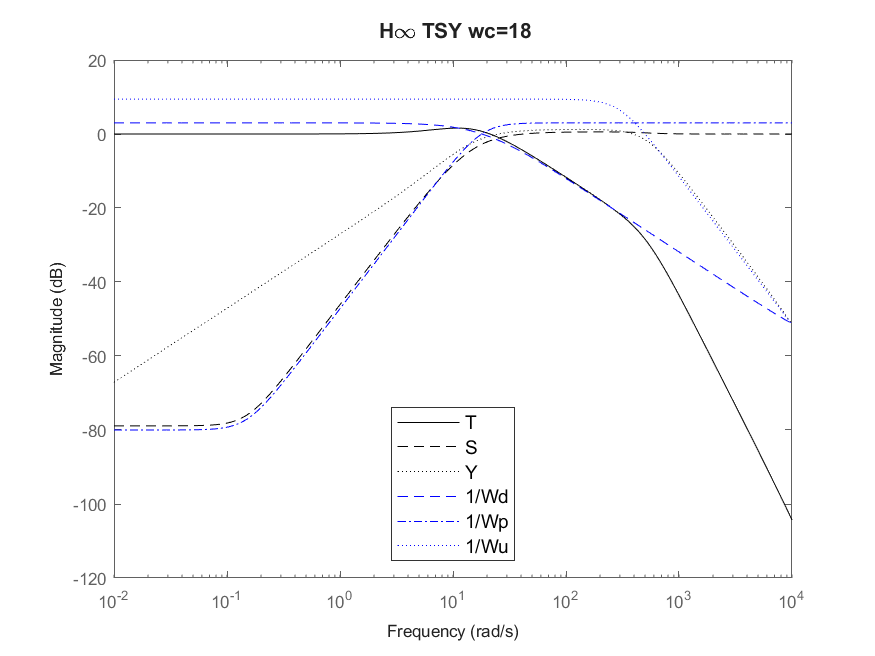
\includegraphics[width=1\linewidth]{Figures/H-TSY-18.png}
    \caption{Closed-loop transfer functions for the $H_{\infty}$-synthesized controller.}
    \label{fig:H-TSY-18}
\end{figure}

For the drive train model and the weights selected, the $H_\infty$ synthesis from \citep{tan2025scaling} achieved $\gamma=1.15$ which is higher than the ideal value of $\gamma<1.00$. This is primarily due to the second-order weighting used on the low-frequency end of $W_p$ and on the high-frequency side of $W_u$, which increases the optimization difficulty but is necessary to produce the desired degrees of sensor noise and disturbance attenuation to outperform other controllers. This sub-optimal $\gamma$ value weakens the guarantees of $H_\infty$ synthesis but is sufficiently low to still provide appropriate loop shaping, as evidenced in Figure \ref{fig:H-TSY-18}. For the $T$ shown in Figure \ref{fig:H-TSY-18}, $T_H(0)=0.99985$, a deficiency of 0.015\%.

Figure \ref{fig:YH-TSY-18} shows the $T$, $S$, and $Y$ transfer functions for the gain-adjusted Youla-H controller. By inspection, it is very similar to the $H_\infty$ Bode plot, with the primary visible change being that $S$ continues to trend downwards with low frequency compared to the $S$ in Figure \ref{fig:H-TSY-18}, which instead plateaus at low frequency.

\begin{figure}[H]
%    \centering
    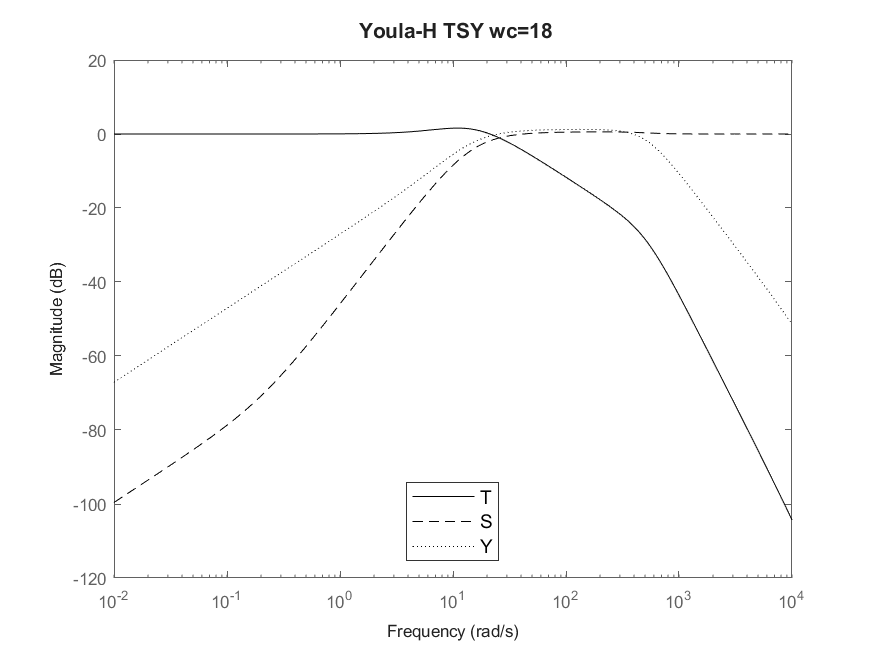
\includegraphics[width=1\linewidth]{Figures/YH-TSY-18.png}
    \caption{Closed-loop transfer functions for the Youla-H controller.}
    \label{fig:YH-TSY-18}
\end{figure}

Since $S+T=1$, the reduction in $S$ at low frequency corresponds to an increase in $T$. We then observe that $T_{YH}(0)=1.00000$.

Most strikingly, Figure \ref{fig:H-YH-Gc-18} compares controller transfer functions, demonstrating that the very small numerical adjustment of $T(0)$ results in significantly different controller characteristics at low frequencies. This is because $G_C=Y/S$, and as $T(0)\rightarrow1.0$, $S(0)\rightarrow0$, resulting in the infinite DC gain at $G_C(0)$ corresponding to a pure integrator.

\begin{figure}[H]
%    \centering
    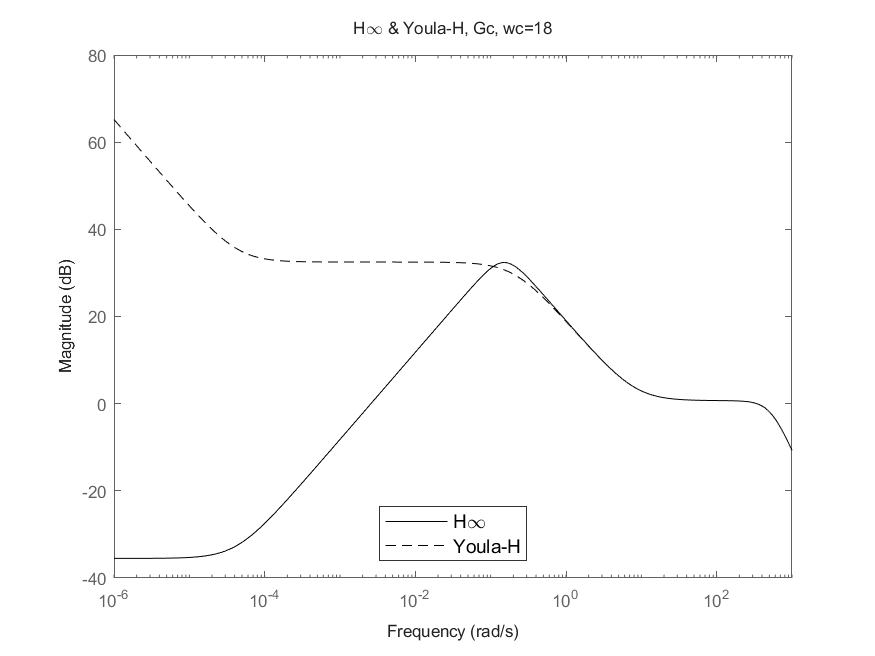
\includegraphics[width=1\linewidth]{Figures/H-&-YH-Gc-18.png}
    \caption{Bode magnitude plot of controller transfer functions $G_C$ for both $H_\infty$ and Youla-H.}
    \label{fig:H-YH-Gc-18}
\end{figure}

Part of the reason for the deficiency in $T(0)$ is that the optimization goal of $\gamma<1.0$ was not met. Due to the control design requirements of our specific system, $\gamma=1.15$ was the best observed outcome. A benefit of the hybrid Youla-H gain tuning method under review is that sub-optimal $\gamma$ values can still result in controllers that satisfy all requirements without having to change weighting functions. However, section \ref{sec:Alternate} showcases that the Youla-H method can still be relevant even with $\gamma<1.0$.

\subsection{Transfer Functions}
Equation \ref{eq:Yh} shows the Youla transfer function for the $H_\infty$-synthesized system.

\begin{equation} \label{eq:Yh}
Y_{H} = 4.5781\frac{(s+8.225) (s+4.316\times10^{-5}) (s^2 + 5.045\times10^{4}s + 1.273\times10^{9})}{(s+1.926\times10^{4}) (s^2 + 25.89s + 216) (s^2 + 721.8s + 2.607\times10^{5})}
\end{equation}

Per the Youla-H method described in this paper, the poles and zeros of this $Y$ are retained when determining the new hybrid $Y$. The 4.5781 DC gain is replaced with a variable DC gain $K$ that is solved in order to ensure $T(0)=1$. The result is the Youla transfer function for the Youla-H system shown below in equation \ref{eq:Yyh}.

\begin{equation} \label{eq:Yyh}
Y_{YH} = \mathbf{4.5787}\frac{(s+8.225) (s+4.316\times10^{-5}) (s^2 + 5.045\times10^{4}s + 1.273\times10^{9})}{(s+1.926\times10^{4}) (s^2 + 25.89s + 216) (s^2 + 721.8s + 2.607\times10^{5})}
\end{equation}

In performing the Youla-H method, the DC gain for $Y$ is shifted by $+0.0114\%$, from 4.5781 to 4.5787. This small change results in the complete removal of accumulating tracking bias with inputs that include ramping profiles.

Equations \ref{eq:Gch} and \ref{eq:Gcyh} show the resulting controller transfer functions for the $H_\infty$ and Youla-H controllers, respectively.

\begin{equation} \label{eq:Gch}
G_{CH} = 4.5781\frac{(s+8.225) (s+4.316\times10^{-5}) (s^2 + 5.045\times10^{4}s + 1.273\times10^{9})}{(s+1.926\times10^{4}) (s^2 + 0.2141s + 0.02291) (s^2 + 747.5s + 2.795\times10^{5})}
\end{equation}

\begin{equation} \label{eq:Gcyh}
G_{CYH} = 4.5787\frac{(s+8.225) (s+4.316\times10^{-5}) (s^2 + 5.045\times10^{4}s + 1.273\times10^{9})}{s(s+1.926\times10^{4}) (s+0.2113) (s^2 + 747.5s + 2.795\times10^{5})}
\end{equation}

The DC gain for both $G_C$ transfer functions are the same as for their $Y$ counterparts. The difference in dynamics between the two controllers is that the low-frequency complex pole pair in $G_{CH}$ is split into a pure integrator and another low-frequency real pole in $G_{CYH}$.

\subsection{Error Comparison}
The error results correspond to tracking performance on the FTP75 drive cycle with the nonlinear drivetrain model. The FTP75 reference input is shown in Figure \ref{fig:FTP75}.

\begin{figure}[H]
%    \centering
    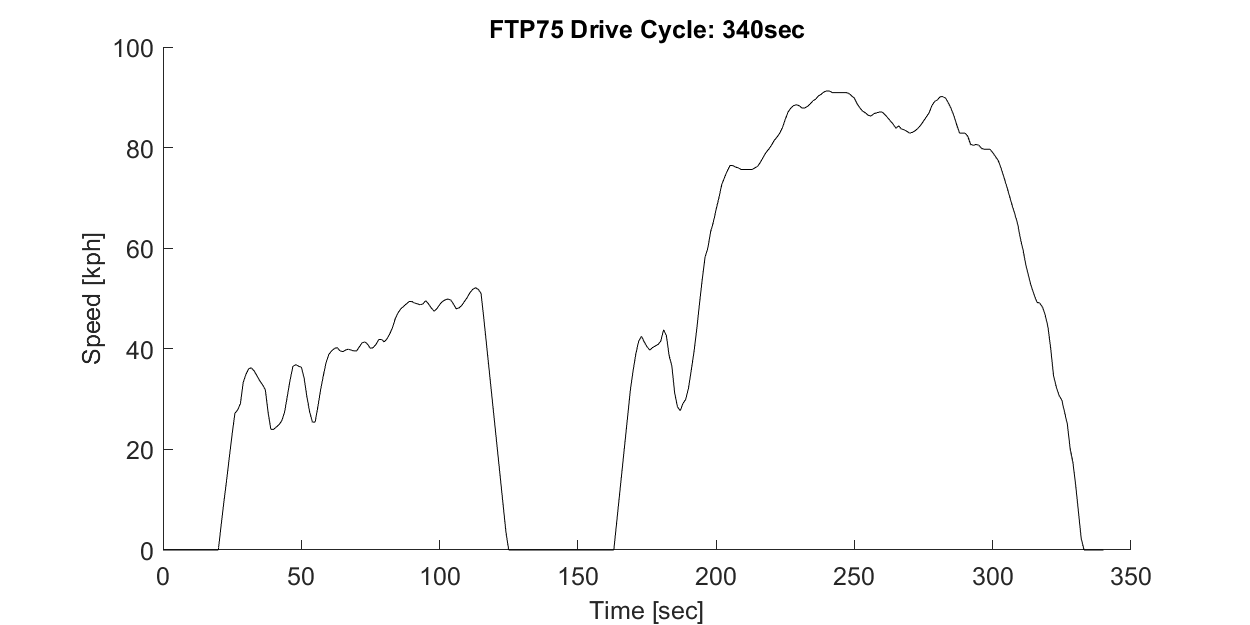
\includegraphics[width=1\linewidth]{Figures/FTP75.png}
    \caption{FTP75 drive cycle.}
    \label{fig:FTP75}
\end{figure}

Figure \ref{fig:H-YH-Err-18} shows the normalized velocity tracking error of the $H_\infty$ and Youla-H drive controllers on the nonlinear plant while tracking the FTP-75 drive cycle.

\begin{figure}[H]
%    \centering
    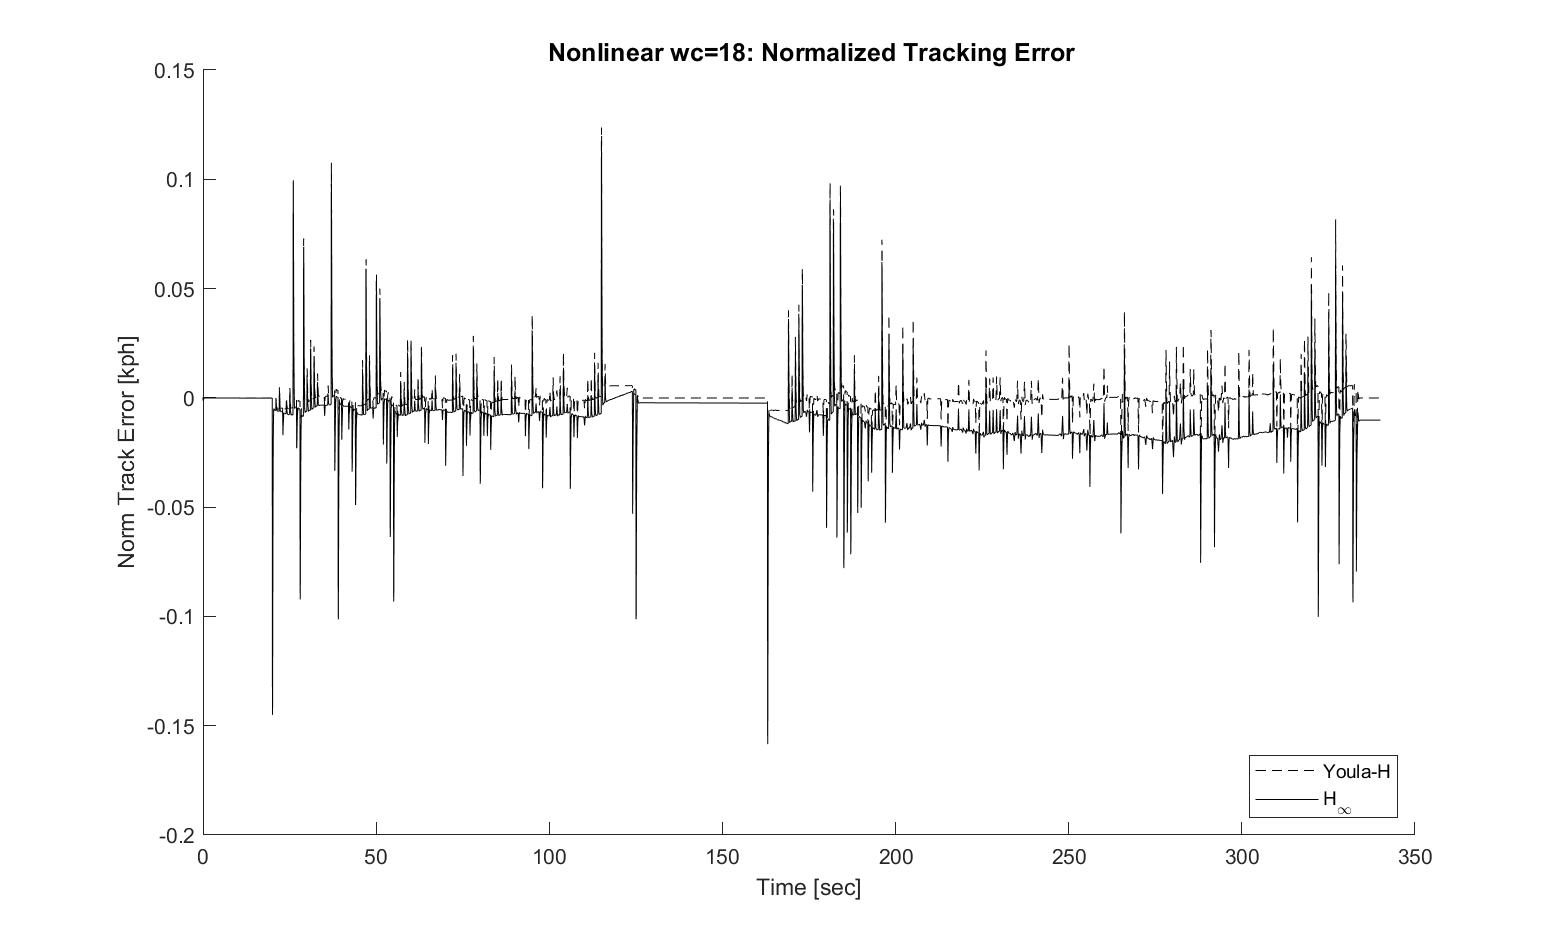
\includegraphics[width=1\linewidth]{Figures/H-YH-Err-18.png}
    \caption{Tracking error of $H_\infty$ and Youla-H drive controllers on nonlinear model.}
    \label{fig:H-YH-Err-18}
\end{figure}

Due to the FTP-75 drive cycle consisting of ramping inputs, the marginal $T_H(0)$ deficiency appears in the tracking results as an accumulating undershoot, while the Youla-H controller has no bias.

Note that the controller bandwidth is high relative to the inputs and disturbances seen in the nonlinear simulation, resulting in spikes of actuator effort and tight tracking. In \citep{tan2025scaling}, this bandwidth was selected across controllers in order to ensure tracking performance and due to the scaled simulation representing a high-power electric vehicle capable of high acceleration. In this paper, the high bandwidth helps to illustrate the accumulating bias clearly.

\subsection{Robustness \& Stability}
The $M_2$ robustness margin, defined as $M_2 = 1 / ||S||_\infty$, is a measure of closed-loop sensitivity to uncertainty that is more comprehensive than gain or phase margins individually, as the $M_2$ margin accounts for combinations of gain and phase margin changes on system stability. The ideal value is $M_2=1.000$. For the $H_\infty$ controller, $M_{2H}=0.937066$, whereas for Youla-H $M_{2YH}=0.937058$, a trivial 0.0008\% reduction in controller robustness.

Since robust control design seeks to provide stability despite uncertainties in model dynamics, stability is likely preserved for sufficiently small perturbations in the Youla gain. However, in general, scaling the Youla parameter modifies the closed-loop pole locations and stability must be verified after gain adjustment. An easy metric is that stability is confirmed when the $M_2$ margin is still greater than zero, assuming the margin is already being calculated.

If a formal validation of stability post-adjustment is required, it must be shown that the new gain does not introduce right-half-plane roots in the system's characteristic polynomial for the given plant model.

\subsection{Alternate System} \label{sec:Alternate}
An alternate system to demonstrate the value of the hybrid Youla-H gain tuning method is shown below in equation \ref{eq:Gp_simple}.

\begin{equation} \label{eq:Gp_simple}
G_{P} = \frac{1}{s+1}
\end{equation}

The weighting functions chosen for this system are all first-order, compared to the second-order slopes used in the drivetrain system. The weighting functions are chosen to be relaxed, allowing for easy optimization, but not so relaxed as to be unrealistic for a controller design problem. Figure \ref{fig:TSY-simple} below shows the weighting functions as well as the resulting closed-loop transfer functions for the simple $G_P$ under review.

\begin{figure}[H]
%    \centering
    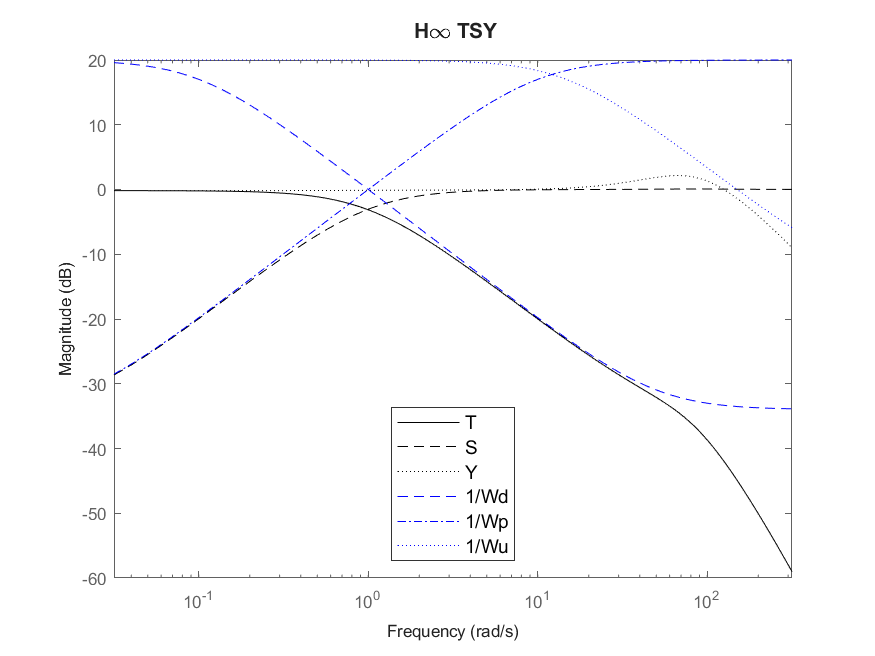
\includegraphics[width=1\linewidth]{Figures/H-TSY-2nd.png}
    \caption{Weighting functions and closed-loop transfer functions for the $H_\infty$ controller on the simple plant.}
    \label{fig:TSY-simple}
\end{figure}

Here, $\gamma = 0.9951$. Despite the optimization succeeding, $T(0) = 0.9999817$, with a deficiency of 0.0018\%. While this is approximately $1/8$ of the deficiency seen for the earlier drivetrain system, it could still present an issue for long-running ramping inputs. Even with a simple plant and relaxed weights, this example serves to demonstrate that the $H_\infty$ optimization under the best-case non-trivial example will typically  still result in minor tracking deficiencies that could be integrated into noticeable tracking bias. The Youla-H method can be utilized even in this easy scenario to fix the closed-loop transfer function DC gains, particularly since code can be reused between projects with minimal modification. See Appendix A for example code.

%%%%%%%%%%%%%%%%%%%%%%%%%%%%%%%%%%%%%%%%%%
\section{Discussion}

This paper presents a practical method of implementing Youla gain-tuning on $H_\infty$-synthesized controllers in order to strictly enforce closed-loop shape characteristics. It presents an alternative to augmenting plant dynamics prior to $H_\infty$ synthesis and is a method that can be readily automated in controller design workflows. Due to the method's flexibility and simplicity, it can be applied by default for control designers utilizing $H_\infty$ control methods. Whether the $H_\infty$ solver succeeds in achieving $\gamma<1.0$ or whether $\gamma$ is reasonably close to $1.0$, any time $H_\infty$ produces a reasonable controller, the Youla-H gain tuning method can be utilized to fix the output controller. In the drivetrain system under analysis in this paper, the gain tuning resulted in a complex pole pair in the $H_\infty$ controller splitting into two real poles, one of which being the required pure integrator to maintain finite steady-state error under ramp inputs.

Preconditions of the Youla-H method are that the plant have a non-zero DC-gain and that the $Y$ transfer function has a non-zero DC-gain. The primary alternative to the Youla-H method would be to augment the plant with an integrator such that the $H_\infty$ algorithm solves for $T(0)=1$ exactly. Due to plant augmentation requiring changes to the plant, it is a less convenient method compared to post-synthesis tuning via Youla methods.

Future work may include investigation into the limits of the Youla-H method, thorough stability analyses, and additions to the types of post-synthesis adjustments that Youla methods can make possible other than simple gain tuning. In the future, an automated controller tuning pipeline could be developed using the Youla-H method as a building block.


%%%%%%%%%%%%%%%%%%%%%%%%%%%%%%%%%%%%%%%%%%
\vspace{6pt} 

%%%%%%%%%%%%%%%%%%%%%%%%%%%%%%%%%%%%%%%%%%
%% optional
%\supplementary{The following supporting information can be downloaded at:  \linksupplementary{s1}, Figure S1: title; Table S1: title; Video S1: title.}

% Only for journal Methods and Protocols:
% If you wish to submit a video article, please do so with any other supplementary material.
% \supplementary{The following supporting information can be downloaded at: \linksupplementary{s1}, Figure S1: title; Table S1: title; Video S1: title. A supporting video article is available at doi: link.}

% Only used for preprtints:
% \supplementary{The following supporting information can be downloaded at the website of this paper posted on \href{https://www.preprints.org/}{Preprints.org}.}

% Only for journal Hardware:
% If you wish to submit a video article, please do so with any other supplementary material.
% \supplementary{The following supporting information can be downloaded at: \linksupplementary{s1}, Figure S1: title; Table S1: title; Video S1: title.\vspace{6pt}\\
%\begin{tabularx}{\textwidth}{lll}
%\toprule
%\textbf{Name} & \textbf{Type} & \textbf{Description} \\
%\midrule
%S1 & Python script (.py) & Script of python source code used in XX \\
%S2 & Text (.txt) & Script of modelling code used to make Figure X \\
%S3 & Text (.txt) & Raw data from experiment X \\
%S4 & Video (.mp4) & Video demonstrating the hardware in use \\
%... & ... & ... \\
%\bottomrule
%\end{tabularx}
%}

%%%%%%%%%%%%%%%%%%%%%%%%%%%%%%%%%%%%%%%%%%
\authorcontributions{Conceptualization, R.T., S.Y. and F.A.; methodology, R.T., S.Y. and F.A.; software, R.T. and S.Y.; validation, R.T. and S.Y.; formal analysis, R.T.; investigation, R.T.; resources, F.A.; data curation, R.T.; writing---original draft preparation, R.T.; writing---review and editing, R.T., F.A. and S.Y.; visualization, R.T.; supervision, F.A.; project administration, F.A.; funding acquisition, F.A. All authors have read and agreed to the published version of the manuscript.}

\funding{This research received no external funding.}

\dataavailability{The original contributions presented in this study are included in the article. Further inquiries can be directed to the corresponding author.} 

\conflictsofinterest{The authors declare no conflicts of interest.} 

% Only for journal Drones
%\durcstatement{Current research is limited to the [please insert a specific academic field, e.g., XXX], which is beneficial [share benefits and/or primary use] and does not pose a threat to public health or national security. Authors acknowledge the dual-use potential of the research involving xxx and confirm that all necessary precautions have been taken to prevent potential misuse. As an ethical responsibility, authors strictly adhere to relevant national and international laws about DURC. Authors advocate for responsible deployment, ethical considerations, regulatory compliance, and transparent reporting to mitigate misuse risks and foster beneficial outcomes.}

% Only for journal Nursing Reports
%\publicinvolvement{Please describe how the public (patients, consumers, carers) were involved in the research. Consider reporting against the GRIPP2 (Guidance for Reporting Involvement of Patients and the Public) checklist. If the public were not involved in any aspect of the research add: ``No public involvement in any aspect of this research''.}
%
%% Only for journal Nursing Reports
%\guidelinesstandards{Please add a statement indicating which reporting guideline was used when drafting the report. For example, ``This manuscript was drafted against the XXX (the full name of reporting guidelines and citation) for XXX (type of research) research''. A complete list of reporting guidelines can be accessed via the equator network: \url{https://www.equator-network.org/}.}
%
%% Only for journal Nursing Reports
%\useofartificialintelligence{Please describe in detail any and all uses of artificial intelligence (AI) or AI-assisted tools used in the preparation of the manuscript. This may include, but is not limited to, language translation, language editing and grammar, or generating text. Alternatively, please state that “AI or AI-assisted tools were not used in drafting any aspect of this manuscript”.}

%\acknowledgments{In this section you can acknowledge any support given which is not covered by the author contribution or funding sections. This may include administrative and technical support, or donations in kind (e.g., materials used for experiments). Where GenAI has been used for purposes such as generating text, data, or graphics, or for study design, data collection, analysis, or interpretation of data, please add “During the preparation of this manuscript/study, the author(s) used [tool name, version information] for the purposes of [description of use]. The authors have reviewed and edited the output and take full responsibility for the content of this publication.”}


%%%%%%%%%%%%%%%%%%%%%%%%%%%%%%%%%%%%%%%%%%
%% Optional

%% Only for journal Encyclopedia
%\entrylink{The Link to this entry published on the encyclopedia platform.}

\abbreviations{Abbreviations}{
The following abbreviations are used in this manuscript:
\\

\noindent 
\begin{tabular}{@{}ll}
MDPI & Multidisciplinary Digital Publishing Institute\\
DOAJ & Directory of open access journals\\
DC & Direct Current\\
\end{tabular}
}

%%%%%%%%%%%%%%%%%%%%%%%%%%%%%%%%%%%%%%%%%%
%% Optional
%\appendixtitles{no} % Leave argument "no" if all appendix headings stay EMPTY (then no dot is printed after "Appendix A"). If the appendix sections contain a heading then change the argument to "yes".
\newpage
\appendixstart
\appendix
%\section[\appendixname~\thesection]{}

\section{Implementation}
MATLAB R2024b was utilized for control design. The code below is an example demonstrating a highly automatable implementation of the Youla-H method using the plant transfer function in Equation \ref{eq:Gp}. The code starts with $H_\infty$ implementation then performs the Youla-H post-synthesis gain adjustment. 

\begin{lstlisting}[style=Matlab-editor, basicstyle=\small\ttfamily]
%% H-infinity controller implementation
% Plant and weighting function transfer functions
Gp = 22.624/(s+4.32e-5);                % Plant transfer function

% makeweight(DC gain, crossover freq, high-freq gain, sample time, slope order)
Wd = makeweight(0.707, 18, 1e3, 0, 1);  
Wp = makeweight(1e4, 18, 0.707, 0, 2);  
Wu = makeweight(0.707, 300, 1e4, 0, 2);

% Perform H-inf controller synthesis
Ph = augw(Gp,Wp,Wu,Wd); % Augmented system for hinfsyn input
[sysGc, Tzw, gamma] = hinfsyn(Ph); % Perform H-infinity synthesis

mreal_tol = 0.001; % Tolerance for minreal for pole/zero pairs
[Gc_n,Gc_d] = tfdata(sysGc); % Reformat output of hinfsyn
Gc_H = zpk(minreal(tf(Gc_n,Gc_d),mreal_tol)); % Hinf Gc

% Construct closed-loop transfer functions
L_H = Gp*Gc_H;
S_H = zpk(minreal(1/(1+L_H),mreal_tol));
T_H = zpk(minreal(L_H/(1+L_H),mreal_tol));
Y_H = zpk(minreal(Gc_H/(1+L_H),mreal_tol));
T0_H = evalfr(T_H,0);                   % Evaluate T(0)

%% Perform Youla-H post-synthesis gain adjustment
syms K, s
[n,d] = tfdata(Gp);
n = cell2mat(n); d = cell2mat(d);       % Reformat output
Gp_sym = poly2sym(n,s)/poly2sym(d,s);   % Construct symbolic Gp

[n,d] = tfdata(Y_H); 
n = cell2mat(n); d = cell2mat(d);       % Reformat output
Y_YH = K*poly2sym(n,s)/poly2sym(d,s);   % Construct symbolic Y_YH
T_YH = simplifyFraction(Y_YH*Gp_sym);   % Construct symbolic T_YH

% Perform gain adjustment
K = solve(subs(T_YH,s,0)-1, K);         % Solve for new gain K
Y_YH = subs(Y_YH);                      % Insert solved K

% Convert back to transfer functions
[n,d] = numden(Y_YH);
Y_YH = zpk(tf(sym2poly(n),sym2poly(d)));
Gc_YH = zpk(minreal(Y_YH/(1-Y_YH*Gp),mreal_tol)); 
T_YH = zpk(minreal(Gc_YH*Gp/(1+Gc_YH*Gp),mreal_tol));
S_YH = zpk(minreal(1/(1+Gc_YH*Gp),mreal_tol));    
T0_YH = evalfr(T_YH,0);                 % Evaluate new T(0)

\end{lstlisting}

%%%%%%%%%%%%%%%%%%%%%%%%%%%%%%%%%%%%%%%%%%
%\isPreprints{}{% This command is only used for ``preprints''.
\begin{adjustwidth}{-\extralength}{0cm}
%} % If the paper is ``preprints'', please uncomment this parenthesis.
%\printendnotes[custom] % Un-comment to print a list of endnotes

\reftitle{References}

% Please provide either the correct journal abbreviation (e.g. according to the “List of Title Word Abbreviations” http://www.issn.org/services/online-services/access-to-the-ltwa/) or the full name of the journal.
% Citations and References in Supplementary files are permitted provided that they also appear in the reference list here. 

%=====================================
% References, variant A: external bibliography
%=====================================
% \bibliography{your_external_BibTeX_file}

%=====================================
% References, variant B: internal bibliography
%=====================================

% ACS format
\isAPAandChicago{}{%
\begin{thebibliography}{999}
\bibitem[Zhou et al.(1996)]{zhou1996robust}
Zhou, K.; Doyle, J.C.; Glover, K. \textit{Robust and Optimal Control}; Prentice Hall: Upper Saddle River, NJ, USA, 1996.

\bibitem[Skogestad and Postlethwaite(2005)]{skogestad2005multivariable}
Skogestad, S.; Postlethwaite, I. \textit{Multivariable Feedback Control: Analysis and Design}, 2nd ed.; Wiley: Chichester, UK, 2005.

\bibitem{assadian2022robust}
Assadian, F.; Mallon, K.R. \textit{Robust Control: Youla Parameterization Approach};
John Wiley \& Sons: Hoboken, NJ, USA, 2022.

\bibitem{tan2025scaling}
Tan, R.; Yadav, S.; Assadian, F. Systemic scaling of powertrain models with
Youla and $\mathcal{H}_\infty$ driver control.
\textit{Energies} \textbf{2025}, \textit{18}, 3126. \url{https://doi.org/10.3390/en18123126}

\bibitem{seatzu2008Hinfint}
Seatzu, C.; Usai, E.; Zaccarian, L. H-infinity controllers with integral action: an experimental evaluation. IFAC Proceedings Volumes, 2008, 41(2), pp. 14,916–14,921.

\bibitem{hu2025YK}
Xiaohai Hu, Jason Laks, Guoxiao Guo, Xu Chen, Iterative Youla-Kucera Loop Shaping For Precision Motion Control. IFAC-PapersOnLine, Volume 59, Issue 30, 2025, pp. 575-580, ISSN 2405-8963

\end{thebibliography}
}

% Chicago format (Used for journal: arts, genealogy, histories, humanities, jintelligence, laws, literature, religions, risks, socsci)
\isChicagoStyle{%
\begin{thebibliography}{999}
\bibitem[Zhou et al.(1996)]{zhou1996robust}
Zhou, K.; Doyle, J.C.; Glover, K. \textit{Robust and Optimal Control}; Prentice Hall: Upper Saddle River, NJ, USA, 1996.

\bibitem[Skogestad and Postlethwaite(2005)]{skogestad2005multivariable}
Skogestad, S.; Postlethwaite, I. \textit{Multivariable Feedback Control: Analysis and Design}, 2nd ed.; Wiley: Chichester, UK, 2005.

\bibitem{assadian2022robust}
Assadian, F.; Mallon, K.R. \textit{Robust Control: Youla Parameterization Approach};
John Wiley \& Sons: Hoboken, NJ, USA, 2022.

\bibitem{tan2025scaling}
Tan, R.; Yadav, S.; Assadian, F. Systemic scaling of powertrain models with
Youla and $\mathcal{H}_\infty$ driver control.
\textit{Energies} \textbf{2025}, \textit{18}, 3126. \url{https://doi.org/10.3390/en18123126}

\bibitem{seatzu2008Hinfint}
Seatzu, C.; Usai, E.; Zaccarian, L. H-infinity controllers with integral action: an experimental evaluation. IFAC Proceedings Volumes, 2008, 41(2), pp. 14,916–14,921.

\bibitem{hu2025YK}
Hu, X.; Laks, J.; Guo, G.; Chen, X. Iterative Youla-Kucera Loop Shaping for Precision Motion Control. arXiv preprint, 2025. (Available: arxiv.org/abs/2508.14309.)

\end{thebibliography}
}{}

% APA format (Used for journal: admsci, behavsci, businesses, econometrics, economies, education, ejihpe, games, humans, ijfs, journalmedia, jrfm, languages, psycholint, publications, tourismhosp, youth)
\isAPAStyle{%
\begin{thebibliography}{999}
\bibitem[Zhou et al.(1996)]{zhou1996robust}
Zhou, K.; Doyle, J.C.; Glover, K. \textit{Robust and Optimal Control}; Prentice Hall: Upper Saddle River, NJ, USA, 1996.

\bibitem[Skogestad and Postlethwaite(2005)]{skogestad2005multivariable}
Skogestad, S.; Postlethwaite, I. \textit{Multivariable Feedback Control: Analysis and Design}, 2nd ed.; Wiley: Chichester, UK, 2005.

\bibitem{assadian2022robust}
Assadian, F.; Mallon, K.R. \textit{Robust Control: Youla Parameterization Approach};
John Wiley \& Sons: Hoboken, NJ, USA, 2022.

\bibitem{tan2025scaling}
Tan, R.; Yadav, S.; Assadian, F. Systemic scaling of powertrain models with
Youla and $\mathcal{H}_\infty$ driver control.
\textit{Energies} \textbf{2025}, \textit{18}, 3126. \url{https://doi.org/10.3390/en18123126}

\bibitem{seatzu2008Hinfint}
Seatzu, C.; Usai, E.; Zaccarian, L. H-infinity controllers with integral action: an experimental evaluation. IFAC Proceedings Volumes, 2008, 41(2), pp. 14,916–14,921.

\bibitem{hu2025YK}
Hu, X.; Laks, J.; Guo, G.; Chen, X. Iterative Youla-Kucera Loop Shaping for Precision Motion Control. arXiv preprint, 2025. (Available: arxiv.org/abs/2508.14309.)

\end{thebibliography}
}{}

% If authors have biography, please use the format below
%\section*{Short Biography of Authors}
%\bio
%{\raisebox{-0.35cm}{\includegraphics[width=3.5cm,height=5.3cm,clip,keepaspectratio]{Definitions/author1.pdf}}}
%{\textbf{Firstname Lastname} Biography of first author}
%
%\bio
%{\raisebox{-0.35cm}{\includegraphics[width=3.5cm,height=5.3cm,clip,keepaspectratio]{Definitions/author2.jpg}}}
%{\textbf{Firstname Lastname} Biography of second author}

% For the MDPI journals use author-date citation, please follow the formatting guidelines on http://www.mdpi.com/authors/references
% To cite two works by the same author: \citeauthor{ref-journal-1a} (\citeyear{ref-journal-1a}, \citeyear{ref-journal-1b}). This produces: Whittaker (1967, 1975)
% To cite two works by the same author with specific pages: \citeauthor{ref-journal-3a} (\citeyear{ref-journal-3a}, p. 328; \citeyear{ref-journal-3b}, p.475). This produces: Wong (1999, p. 328; 2000, p. 475)

%%%%%%%%%%%%%%%%%%%%%%%%%%%%%%%%%%%%%%%%%%
%% for journal Sci
%\reviewreports{\\
%Reviewer 1 comments and authors’ response\\
%Reviewer 2 comments and authors’ response\\
%Reviewer 3 comments and authors’ response
%}
%%%%%%%%%%%%%%%%%%%%%%%%%%%%%%%%%%%%%%%%%%
\PublishersNote{}
%\isPreprints{}{% This command is only used for ``preprints''.
\end{adjustwidth}
%} % If the paper is ``preprints'', please uncomment this parenthesis.
\end{document}

